% Added by BB
%% This holds definitions of macros to enforce consistency in names.

% This file is the sole location for such definitions.  Check here to
% learn what there is and add new ones only here.  

% also see units.tex for units.  Units can be used here.

%%% Common terms

% Check here first, don't reinvent existing ones, add any novel ones.
% Use \xspace.

%%%%% Anne adding macros for referencing CDR volumes and annexes Apr 20, 2015 %%%%%
\def\expshort{DUNE\xspace}
\def\explong{The Deep Underground Neutrino Experiment\xspace}

\def\volintro{CDR Volume 1: Introduction\xspace}
\def\volphys{CDR Volume 2: Physics with DUNE at LBNF\xspace}
\def\vollbnf{CDR Volume 3: LBNF\xspace}
\def\voldune{CDR Volume 4: The DUNE Detectors\xspace}

\def\anxcernproto{Annex: CERN Single-phase Prototype Detector Proposal\xspace}
\def\anxlbnefd{Annex: LBNE FD Design Jan 2015\xspace}
\def\anxrates{Annex: Data Rates\xspace}
\def\anxndref{Annex: Near Detector Reference Design\xspace}
\def\anxlbnoa{Annex: LAGUNA/LBNO Part 1\xspace}
\def\anxlbnob{Annex: LAGUNA/LBNO Part 2\xspace}
\def\anxlbnesci{Annex: LBNE: Exploring Fundamental Symmetries of the Universe\xspace}
\def\anxdualrpt{Annex: Progress report on LBNO-DEMO/WA105 (2015)\xspace}
\def\anxdualtdr{Annex: WA105 TDR\xspace}

\def\cernsingleproto{Name of CERN Single-Phase Prototype\xspace}
\def\cerndualproto{Name of CERN Dual-Phase Prototype\xspace}

% Things about oscillation
%
% example: \dm{12}
\newcommand{\dm}[1]{$\delta m^2_{#1}$\xspace}
% example \sinstt{12}
\newcommand{\sinstt}[1]{$\sin^22\theta_{#1}$\xspace}
% example \deltacp
\newcommand{\deltacp}{$\delta_{\rm CP}$\xspace}
% example \nuxtonux{\mu}{e}
\newcommand{\nuxtonux}[2]{$\nu_{#1} \to \nu_{#2}$\xspace}
\newcommand{\numutonumu}{\nuxtonux{\mu}{\mu}}
\newcommand{\numutonue}{\nuxtonux{\mu}{e}}
\newcommand{\numu}{$\nu_\mu$\xspace}
\newcommand{\nue}{$\nu_e$\xspace}
\newcommand{\anumu}{$\bar\nu_\mu$\xspace}
\newcommand{\anue}{$\bar\nu_e$\xspace}

% Names
\newcommand{\cherenkov}{Cherenkov\xspace}
\newcommand{\kamland}{KamLAND\xspace}
\newcommand{\kamiokande}{Kamiokande\xspace}
\newcommand{\superk}{Super--Kamiokande\xspace}
\newcommand{\miniboone}{MiniBooNE\xspace}
\newcommand{\minerva}{MINER$\nu$A\xspace}
\newcommand{\nova}{NO$\nu$A\xspace}
\newcommand{\SURF}{Sanford Underground Research Facility\xspace}

\def\Ar39{$^{39}$Ar}
\def\driftvelocity{\SI{1.6}{\milli\meter/\micro\second}\xspace}

%\begin{document}
% PLEASE FOLLOW POSTED GUIDELINES!!

% Please see the two LAr CDR 'guidelines' writeboards in basecamp
% at https://lbne-doc.basecamphq.com/projects/4264323/writeboards
% One is for text, the other for images and figures 

\chapter{Alternatives Not Selected} %AH changed 2/6/12
\label{ch:alternatives}

Alternative detector configurations and design parameters %\fixme{
that were considered but ultimately rejected for other designs are discussed in this chapter.

%%%%%%%%%%%%%
\section{Detector Configuration}
\subsection{Double Phase Readout}

The European GLACIER collaboration is pursuing a novel double-phase readout detector technology that has potential advantages. In this scheme, ionization electrons are drifted upwards under the influence of an electric field towards the liquid-vapor interface. The electrons are extracted from the liquid into the vapor by an electric field of 2.5~kV/cm. The electrons then drift to two stages of Large Electron Multipliers (LEM). Electrical signals are induced on segmented electrodes on the LEM. 

This method requires far fewer readout channels than %the preferred 
our reference design, however significant R\&D is required to demonstrate the viability of this technique for a large detector. This design requires very long electron-drift lengths ($\sim$ 20m) in order to be cost-effective.

\subsection{Cryostat Shape}

Storage tanks can be classified by shape (upright cylinder, horizontal cylinder, rectangular parallelepiped) and means of support (self supporting, externally supported).

A horizontal cylindrical tank would require significant structural support to withstand the gravitational load.  On the other hand, upright self-supporting cylindrical tanks are commonly used for surface storage of cryogenic liquids. The proposed above-ground LArTPC experiment FLARE utilized a tank of this configuration. An upright cylindrical tank is also proposed for the 100-kton GLACIER underground detector. In contrast, the 600-ton ICARUS detector is a rectangular parallelepiped. 

A study was performed~\cite{docdb355} to compare the cost for three configurations of equivalent active mass: upright cylindrical cryostat (soup can), rectangular parallelepiped externally-supported cryostat (membrane) and the rectangular parallelepiped self-supporting cryostat (modular). The study considered the cost of rock excavation, the cost of the total inventory of LAr required for a detector with a fixed active mass and a rough estimate of the cryostat cost. 

The active/total mass fraction for the three configurations ranges between 70\% and 74\% and is therefore not a significant factor in the cost difference. The major cost factor is the volume of rock that must be excavated for these configurations. There is a significant amount of unused cavern space if an upright cylindrical tank is located within a rectangular parallelepiped cavern. The amount of unused space can be reduced by excavating a cylindrical cavern but the excavation cost would increase significantly ($\sim$ 30\%).

The study results show a cost range of 10\% - 20\% for the different configurations. This is within the uncertainty of the estimates ($\sim$ 50\%) so none of the options can be rejected purely on economic grounds given our current state of knowledge. Given sufficient resources, all configurations could be more fully developed to make a more informed decision, however any potential value would be offset by the cost of pursuing multiple design paths. 

The study results also indicate that a membrane cryostat is the most cost-effective solution. It clearly maximizes the use of the excavated rock volume. A membrane cryostat is also inherently more cost-effective than a self-supporting cryostat since the hydrostatic pressure of the liquid is constrained by the cavern walls and not the cryostat walls, thereby reducing the amount of structural steel required.

\subsection{Modular Cryostat}

The modular LANNDD detector %%%%%%%   STILL TO ADDRESS          \fixme{ref} 
concept was considered. % and rejected. 
The main benefit of the LANNDD concept is that the cryostat is evacuable. However, reinforcing members within the cryostat would be required to withstand the vacuum load. Physics cuts around these members would reduce the fiducial mass of the detector significantly relative to the membrane-cryostat reference design. Results from the Liquid Argon Purity Demonstrator %%%%%%%   STILL TO ADDRESS          \fixme{ref} 
have shown that cryostat evacuation is not required to achieve excellent LAr purity.

%%%%%%%%%%%%%
\section{Depth Options}

\subsection{Surface and 300L}

Cosmic-ray backgrounds for accelerator-based neutrino analyses are negligible in an LArTPC located on the surface of the earth. The cosmic-ray rate on the top of an APA drift cell of size 2.5~m $\times$ 5~m would be 2~Hz if it were located at the surface. A neutrino event is fully contained within the drift cell and the drift time is 1.5~msec, so the rate of accidental cosmic rays in a drift cell containing a neutrino event is 0.2\%.  The physics scope of either the surface
or 300L options would be restricted to accelerator neutrinos since a competitive proton-decay search could not be performed with such a high background rate. The cost of underground construction is significantly higher than conventional surface construction so there is no clear benefit from the 300L option. 

Significant cost savings (several \$100M) would result for the surface option.  However, space charge build up due to the relatively high cosmic ray flux on the surface and the slow ion drift velocity may result in unacceptable distortions in the electric field using the long 3.7 m drift that is planned for the LAr-FD.  This can be mitigated by reducing the drift length, which would result in a substantial increase in the number of channels and a modest reduction in the ratio of fiducial volume to total volume.  These would, in turn, increase the cost of the detector, partially offsetting the cost reduction from moving to the surface.

\subsection{800L}

In addition to the reference design described in this CDR for a LAr-FD at the 4850L, a candidate design for the 800L was also developed \cite{docdb4314}.  At this depth, there is an unacceptable level of background to $p \rightarrow \nu K^+$ due to the creation of K0L by cosmic ray muons in the surrounding rock, which subsequently charge exchange within the LAr detector to create an isolated $K^+$.  To mitigate this effect, a large-area veto system was included in the 800L design, in order to tag muons which could generate such background and thereby eliminate candidate proton decay events in coincidence with a detected muon.  Given the goal of essentially zero background for the proton decay search (\cite{bueno-pdk} quotes a background rate on the order of 1 event in 30 years), the veto system would be required to be extremely efficient, and therefore essentially completely hermetic.  However, due to the practical engineering considerations of how to implement a veto system extending 7 m into the rock at both top and bottom of the main detector, it proved difficult to achieve the required hermetic coverage.  In addition, at the position of the proposed cavern at the 800L, the cosmic ray flux – angle and energy – depend on the details of the surface topography, which would require extensive simulations to be able to be assured of the efficacy of the veto system for reducing the background to the required level.  Moving the detector to the 4850L reduces the cosmic ray background by three orders of magnitude, essentially eliminating these concerns.

Cosmic ray muons passing through the LAr detector itself can produce spallation products with lifetimes too long to allow signals resulting from their subsequent decay to be vetoed by observing the muon that created them.  These would create backgrounds that could compromise low-energy physics searches, of which the observation of neutrinos from a distant core-collapse supernova is the prime, but not only example.  The spectrum of spallation products of argon is not well known, nor is the spectrum of low-energy searches that the LBNE LAr-FD may be called upon to do, so it is difficult to quantify the effect of such background.  Since the spallation backgrounds cannot be vetoed, the only way to reduce them is to move the detector to greater depth.

Based on these considerations, as well as the fact that siting LBNE at the 4850L would help enable other deep underground science in the U.S., the LBNE Collaboration Executive Committee, in its meeting in December 2011, issued a statement that ``There was a very strong preference for siting the experiment at the 4850L depth.''

%%%%%%%%%%%%%
\section{Cryogenics Plant}


\subsection{LAr Supply using a Temporary Air-Separation Plant}

We have considered whether the provision of a temporary, dedicated air-separation plant could be justified based on the elimination of LAr losses due to boil-off during transportation, elimination of vehicle movements and the potential increase in the supply reliability. These advantages must be offset against the net capital cost of the temporary plant, the operating cost of the plant and the relative inefficiency of the small temporary plant as compared to a large commercial plant. We have been advised by LAr suppliers that this would not be cost-effective.

\subsection{LAr Storage}

It would be desirable to provide temporary storage of LAr to decouple the delivery schedule from the detector construction schedule. Ideally, temporary storage could reduce the schedule by six months since argon deliveries can occur in parallel with detector construction. This is only possible if construction of the temporary storage facility occurs concurrently with other activities.

Temporary storage would also mitigate the risk of a detector failure necessitating access to the cryostat. If a sudden detector-wide failure occurred and temporary storage were not available, the argon would be vented to the atmosphere and the \$25M investment of LAr would be lost. The cryostat filling sequence described in Chapter~\ref{ch:install} %this report 
effectively eliminates the likelihood of failure during detector commissioning. A sudden detector-wide failure occurring during operations is highly unlikely. It is more likely, but still unlikely, that a gradual degradation of detector performance would occur over an extended period of time, allowing time for a decision to be made to construct a storage tank.



\subsection{Common Riser for LAr and LN}

%%%%%%%   STILL TO ADDRESS          \fixme{say what a 'riser' is}
The potential for the replacement of the two liquid cryogen risers (LAr and LN) with
 a common cryogenic riser may be considered during later design phases. The fill lines are not
 normally used during operation. After initial filling of the cryostat the argon line is not planned
 to be used unless the cryostat is to be drained. The common line would be configured in standby
 mode for LN service in case of unplanned outage of the refrigeration plant.

%%%%%%%   STILL TO ADDRESS          \fixme{if this is still `on the table' should it be in chapter 2?}

\subsection{Common Vent Lines}

A common vent system could be adopted that would be suitable for both nitrogen and
 argon. It would need to be sized for the peak combined flow rate. The probability of either argon
 or nitrogen being vented under normal operations is low, but a Simultaneous Operations Study
 (SIMOPS) would be required to demonstrate that cross-contamination could not occur during
 commissioning, or normal or emergency operations. A greater level of design detail is required to
 support this study than has been possible to-date and therefore separate vents have been included
 at this stage.

%%%%%%%   STILL TO ADDRESS           \fixme{ditto: if this is still `on the table' should it be in chapter 2?}


%%%%%%%%%%%%%
\section{Cryostat Insulation}
%\subsection{Insulation}

The original LANNDD modular cryostat included the use of a vacuum-insulated space between the inner and outer tanks, resulting in a significant decrease in the required refrigeration
load. This benefit would need to be weighed against the added capital cost of a vessel that can
withstand the vacuum load. Arup eliminated the vacuum-insulated option during the screening
process, citing the benefit of not having an outer tank designed for a full vacuum load.

The use of a vacuum-jacketed cryostat was rejected. The most serious concern is an accident scenario that would result in a significant leak in the inner vessel. The outer tank and the argon venting system would need to be designed to cope with the large volume of released gas.

%%%%%%%%%%%%%
\section{TPC}
\subsection{TPC Configuration}

\subsubsection{Reference Design 1a}

The first proposed Reference Design, 1a, relied on a minimal extrapolation of the MicroBooNE TPC module design. % \fixme{ref}. 
The detector would be installed in a cavern with drive-in access and would consist of a rectangular stack of TPC modules that had been constructed above-ground.

A modest extrapolation of the MicroBooNE module design parameters does not introduce large cost uncertainty if done properly. The extrapolations are in dimensions that do not challenge the limits of the technology. Rather, this detector configuration suffers from a poor fiducial/total mass fraction. Only 56\% of the LAr in the detector would be useful for physics and the cost is $\sim$3 times the cost of the selected reference design.

\subsubsection{Reference Design 2a}

Reference Design 2a is similar to the selected reference design. The major difference is the use of room-temperature, accessible electronics. The concept is shown in Figure~\ref{fig:refdes2a}.

\begin{figure}[h]
\centering
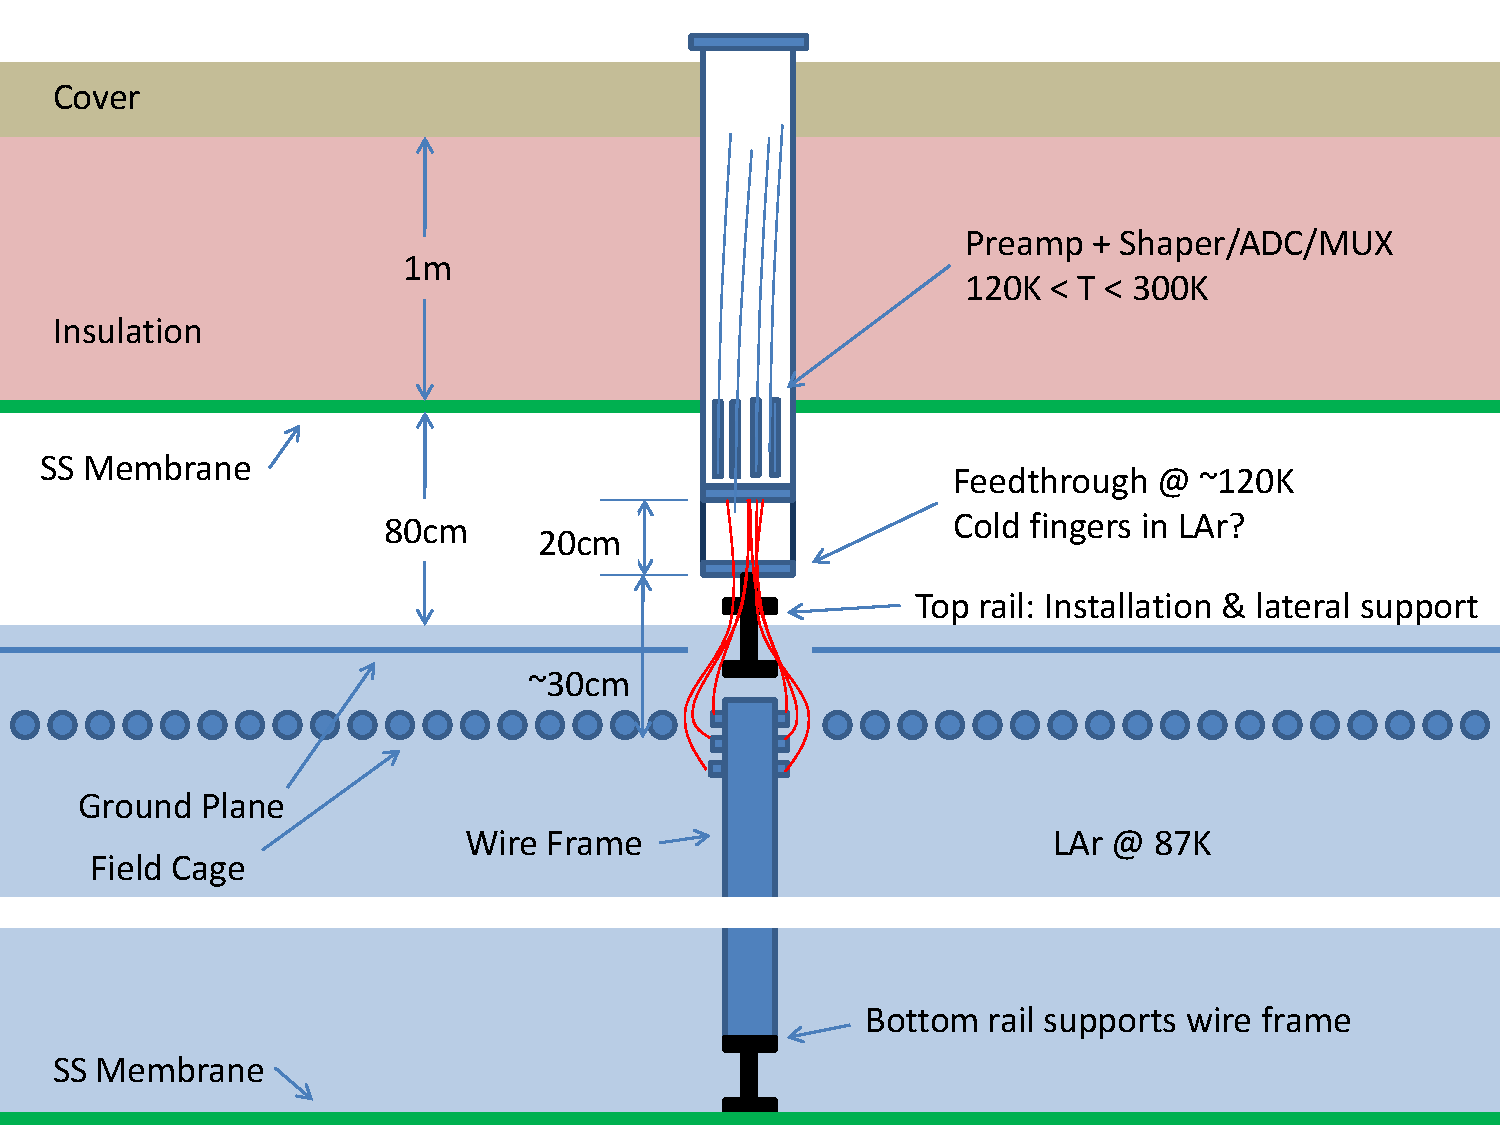
\includegraphics[width=\textwidth]{v5ch08_refdes2a}
\caption[Alternate cable routing from an APA to a cold feedthrough]{Reference Design 2a, showing cable routing from an Anode Plane Assembly to a cold feedthrough. The warm readout electronics are located within the feedthrough. }
\label{fig:refdes2a}
\end{figure}

Short low-impedance cables route wire signals from the Anode Plane Assemblies (APAs) to a cold feedthrough which is kept at $\sim$ 120~K. The readout electronics are located within the feedthrough. The benefit of this design is that the electronics boards can be replaced without removing LAr from the detector.

There are a number of disadvantages to this concept, however. The cable lengths must be kept to $\sim$ 1~m,  the wire spacing must be increased to 5~mm and the wire angle reduced from $45^{\deg}$ to $30^{\deg}$ in order to achieve a marginally acceptable signal-to-noise ratio. As a result, the track resolution in the vertical direction is $\sim$ 1~cm. A large number of feedthroughs are required in order to keep the cable lengths short. One feedthrough containing 576 electronics channels is required for every 53~cm along the top of each APA. Each feedthrough would be 34~cm $\times$ 22~cm in cross section and would be $\sim$ 2~m long.

\subsection{Wire Spacing}

The distinguishing feature of the LArTPC is the ability to distinguish one MIP electrons from 2 MIP electron-positron pairs close to the interaction vertex. A wire spacing smaller than the design (5~mm) would have smaller signal-to-noise ratio (S/N) commensurate with the wire spacing. The design S/N ratio could be restored by decreasing the noise. The most direct means of accomplishing this would be to reduce the wire length, thereby increasing the number of electronics channels. Reducing the wire spacing below 5~mm will only offer minimal benefit since the background from NC$\pi^0$ events is already quite small. 

\subsection{Number of Wire Planes}

The reference design includes three instrumented wire planes and one un-instrumented grid plane. Reducing the number of instrumented planes to two would reduce the detector cost by $\sim$\ \$3M with a negligible loss of $\nu_e$ identification efficiency. This would also reduce the readout redundancy, however, and potentially affect the long-term reliability of detector operations. We do not consider this a credible value-engineering option.

The un-instrumented grid plane could be eliminated, saving $\sim$\ \$1M. The grid plane is used to create equal signal levels in both induction planes. The signal level in the first induction plane would be reduced by $\sim$2 times if the grid plane were eliminated. The grid plane also provides electrostatic discharge protection for the instrumented wires.
We do not consider this a credible value-engineering option.

\subsection{Drift Length}

Selection of the design drift length is highly coupled with the expected LAr purity, the wire spacing and the required $\nu_e$ identification efficiency and background rejection. The ICARUS detector is currently operating with a drift electron lifetime of 6  to 7~ms. We expect the LAr purity in LAr-FD to be equal or superior to ICARUS. Increasing the drift distance beyond the reference design of 3.7~m would result in significant cost savings. The 5~mm wire spacing is well matched to this drift distance; it is roughly twice the transverse diffusion RMS. As an example, if the drift distance were increased to 5~m, the wire spacing could be increased to $\sim$ 6~mm. The minimum signal-to-noise ratio would suffer a minor decrease from 36:1 to 30:1 if the electron lifetime was 6~ms. The effect of such a change on physics analyses has not yet been explored.

%%%%%%%%%%%%%
\section{DAQ Cable Routing} % title changed
%%%%%%%%%%%%%

The concept of routing raw signals from all wires out of the cryostat, as ICARUS does, was considered.% and rejected. 
The large data rate would require a huge number of cables and feedthroughs with little benefit since the vast majority of the sampled wire signals have no information. The large cable plant would be a major contributor to LAr impurities.

\section{Installation \& Commissioning}
%%%%%%%%%%%

The initial Installation and Commissioning concept was to support the %detector \fixme{the 
TPC on the floor of the cryostat. Cross-bracing in both directions would be required to ensure mechanical stability and would compromise the TPC design. Hard points in the cryogenic insulation would be needed  which would likely require design modifications to the standard vendor-supplied membrane-cryostat insulation system. 

Several alternatives for accessing the top of the detector during installation were considered. A scissors lift was considered and rejected due to concerns that the lift could sway and damage detector components. Consideration was given to a moveable platform that would traverse the top of the detector on rails, or alternatively, using a temporary catwalk. These systems would provide access to the top of the detector but not at intermediate heights.

Several installation sequences were considered; row-wise versus column-wise installation of APAs and CPAs. The current installation sequence was deemed superior in that it minimizes work activities in previously installed sections of the detector. This reduces the risk of damage during installation.

\section{Photon Detection}

Most LArTPCs use TPB-coated PMTs to detect scintillation light. Light emitted more than a few meters from a PMT is diffused by Rayleigh scattering ($\lambda \approx$ 90~ccm), so PMTs would need to be placed between drift cells. This configuration is not compatible with the APA concept. Conceptually, each interior cathode plane can be replaced with two cathode planes separated by sufficient space for an array of PMTs. This would increase the width of the detector and the cavern by $\sim$ 1m and result in a lower fiducial mass.

A variety of options were considered for the wavelength-shifting scheme and the light guides. These options suffer from lower light-collection efficiency and result in higher cost for the same performance.

\section{LAr1 Prototype}

A variety of alternatives to the LAr1 prototype have been considered, e.g. constructing a series of smaller prototypes to validate the integration of the detector systems. 
However, smaller prototypes may not catch some unknown issues that this technology, in its current state of maturity, may present.
